\documentclass{article}

\usepackage[mathcal,mathbf]{euler}
\usepackage{theorem,amsmath,enumerate,fancyhdr,amssymb,amsfonts}
\usepackage[pdftex]{graphicx}

\usepackage{myDefs}
\usepackage{undertilde}

\title{ 
    Algorithmic Learning Theory\\
    Spring 2017\\
    Lecture 3
}

\author{
    {\bf Instructor:} Farid Alizadeh\\
    {\bf Scribe:} Atharv Bhosekar\\
    {\bf Edit:} Yuan Qu\\
}

\date{02/01/2017}

\begin{document}

\pagestyle{fancy}

\lhead{
    {\bf Scribe: }{Atharv Bhosekar }
    {\bf Edit: }{Yuan Qu}\\
    {\bf Lecture 3}
}

\rhead{
    {\bf Date: }{02/01/2017}
}

\maketitle

\medskip

This lecture introduces k-Nearest Neighbor (k-NN) method and discusses the following:  

% \begin{enumerate}
%     \item k-NN overview 
%     \item k-NN for regression
%     \item key features of k-NN
%     \item notion of nearness
%     \item voronoi diagrams
%     \item computational complexity of k-NN
%     \item Issue with high number of features
% \end{enumerate}

\begin{enumerate}
    \item Overview
    \item Application Methods
        \begin{enumerate}
            \item k-NN for Bayes
            \item k-NN for regression
        \end{enumerate}
    \item Properties
        \begin{enumerate}
            \item Non-parametric
            \item Distance
            \item Standardization
        \end{enumerate}
    \item Validation (in Lecture 4)
\end{enumerate}     

\clearpage 

\section{Overview}{
    k-NN, a classification method, as the name suggests, takes k nearest points in the available data set to the desired new point, averages the responses for those points and reports that as the response at the new point. 

    Supposed that we have a data set following:

    \begin{center}{
        \begin{tabular}{c|c c c c }

            $y$ & $x_1$ & $x_2$ & ... & $x_p$ \\
            \hline
            $y_1$ & $x_{11}$ & $x_{12}$ & ... & $x_{1p}$ \\
            
            $y_2$ & $x_{21}$ & $x_{22}$ & ... & $x_{2p}$ \\
            
            ... & ... & ... & ... & ... \\
            
            $y_n$ & $x_{n1}$ & $x_{n2}$ & ... & $x_{np}$ \\
            
        \end{tabular}
    }
    \end{center}

    The problem is to find the output $y_{new}$ for a new input \(x_{new}=(x_1,x_2, \cdots,x_p)\). k-NN method suggests that:

    \[y_{new}=\frac{\sum y \text{ of } k \text{ nearest points}}{k}\]

    \[\Rightarrow P[y_{new}=i]=\frac{\text{number of } y_j=i}{k}, j=1,2,\cdots,k\]

    In two demension, if there are two classes, \(y=0\) and \(y=1\), so:

    \[P[y=0|x]=\frac{f_{x|y}(t|0)P[0]}{f_x(t)}\]

    If $x$ is in IID (Independent and Indentical distribution), we have:

    \[f_{x|y}(t|0)\approx \frac{f(t_{[1]}|0)+\cdots+f(t_{[k]}|0)}{k}, t_{[i]} \text{ is the $i$th closest number to the $t$}\]

    \paragraph{e.g. }{
        To better visualize this, consider an example of a classification problem with two features, $x_1$ and $x_2$, and two classes, blue and black, as shown in Figure \ref{Fig.1}. 

        \begin{figure}
            \label{Fig.1}
            \begin{center}
                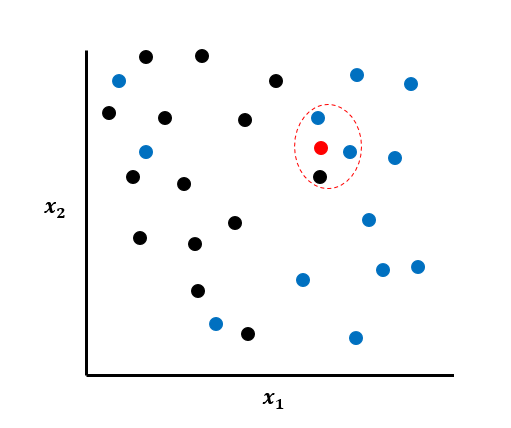
\includegraphics[scale=0.5]{classificationkNN.PNG}
                \caption{Example of a 2 feature 2 class classification problem. Red point shows the point to be classified. Points in the red dotted circle denote 3 nearest neighbors.}
            \end{center} 
        \end{figure}

        The problem is to classify the new point (the red point) as blue or black. 

        For illustration, consider $k = 3$ i.e. consider three nearest neighbors to the new point. 

        Three points shown in the circle are found to be closest to the new point, 2 blue 1 black. Taking average of three points, the new point is 2/3rd likely to be blue and 1/3rd likely to be black. Therefore,the k-NN algorithm classifies the new point as blue. 

        (some question about it) One small point to notice here is that the class reported based on k-NN is the class that has maximum value and does not take in to consideration the magnitude by which that class is favored over the other class.
    }
}

\section{Application Methods}{
    \subsection{k-NN for Bayes}{
        Considering Bayes' decision rule, with a vector of features \(\utilde{x} = (x_1, x_2, \dots, x_p)\), where $p$ is the number of features. The problem is to find \[y_{\mathrm{new}} = \underset{y}{\mathrm{argmax}}\, P[y|\, \utilde{x}_{\mathrm{new}}]\]

        To put it in words, given a new point $x$, the problem is to find the probability that it belongs to the class relevant to the problem. But the probability may be uncomputable because of infinity of points.

        k-NN solves this problem by making two assumptions: 
        \begin{enumerate}
            \item Replace \(\utilde{x}_{\mathrm{new}}\) with k-neighbors of \(x_{\mathrm{new}}\). 
            \item Approximates \(P \approx \) proportion of the neighborhood in each class.
        \end{enumerate}
        
    }
    \subsection{k-NN for regression}{
        Loss function :\(\mathrm{loss}(x, \hat{f}\,|\,f) = (f(x) - \hat{f}(x))^2 \rightarrow \) Square error.



        \[\mathrm{risk}(\hat{f}\,|\,f) = E_x \cdot \mathrm{loss}(x, \hat{f}\,|\,f) = E_x(f(x) - \hat{f}(x))^2\]

        Assuming we have the entire population, best \(\hat{f}\) is given by \(\hat{f} = E_x(y)\), so we have:

        \[\hat{f}(x_{\mathrm{new}}) = \text{average of all } \{y\,|\,x=x_{\mathrm{new}}\}\]

        which maybe uncomputable because of infinity of points (need to get all \({y\,|\,x = x_{\mathrm{new}}}\)).

        In this case, the error is caculated by square error, which the average leads to the minimum value, while median minimize the absolute error.

        k-NN solves this problem by making two assumptions:
        \begin{enumerate}
            \item Replace \(x_{\mathrm{new}}\) with closest $k$ neighbors $x_i$ of \(x_{\mathrm{new}}\). 
            \item The average of all $y$ at \(x_{\mathrm{new}}\) is approximated by $y_i$ of the k-nearest neighbors.
        \end{enumerate}

        If the loss function change to absolute function, the average should change to median.
    }
}

\section{Properties}{
    \subsection{Non-parametric}{
        k-NN is a purely non-parametric method. This can be derived from the observation that the loss function in case of both classification as well as regression does not make any assumption on the nature of surrogate function $\hat{f}$.
    }
    \subsection{Distance}{
        Entire k-NN method is dependent on finding and utilizing k-nearest neighbors. However, there are some issues that one needs to take in to account while defining nearness. 

        It is important to note that the operation on the responses of $k$ nearest neighbors to obtain the response at a new point is dependent on the loss function. For example, average is used only if the loss function is squared error, median will be used if the loss function is sum of absolute values and so on.

        If all $x_i$ are numerical, then,

        \[\text{Eucliden distance: }\| \utilde{a} - \utilde{b}\| = \sqrt{\sum_{i=1}^{p}(a_i - b_i)^2}\]

        \[\text{Manhatten distance: }\| \utilde{a} - \utilde{b}\| = \sum_{i=1}^{p}|a_i - b_i|\]

        \[\text{Minkowski distance: } l_r \text{ distance}\begin{cases}
            r=0  &  \text{Number of items} \\
            r=1  &  \| \utilde{a} - \utilde{b}\| = \sum_{i=1}^{p}|a_i - b_i| \rightarrow \text{Manhatten distance} \\ 
            r=2  &  \| \utilde{a} - \utilde{b}\| = \sqrt{\sum_{i=1}^{p}(a_i - b_i)^2} \rightarrow \text{Eucliden distance} \\ 
            r  &  \| \utilde{a} - \utilde{b}\| = \sqrt[r]{\sum_{i=1}^{p}(a_i - b_i)^r} \\ 
            r\rightarrow \infty  &  \| \utilde{a} - \utilde{b}\| = \mathit{max} \{|a_i - b_i|\}
        \end{cases}\]
        
        If all $x$ is categorical, \(x \rightarrow \{A,B,\cdots,L\}\) then,
        \[\| x - y\| = \begin{cases}
            0,  &  \text{if same class}\\
            1,  &  \text{otherwise}
        \end{cases}\]
        Hamming distance: \(| "a_1a_2\cdots a_m" - "b_1b_2\cdots b_m" |\)

        \paragraph{Voronoi diagrams}{
            Voronoi diagrams use the principle of k-NN in the sense that it divides the space based on the nearest sample (or one nearest neighbor) of point. 

            For example, if one has two data points in the space, the space is divided in to two halfspaces from the mid-point of those two data points. Similarly, k-level voronoi diagrams use the principle of k nearest neighbors. A sample Voronoi diagram is shown in Figure \ref{Fig.2}.
            \begin{figure}
                \label{Fig.2}   
                \begin{center}
                    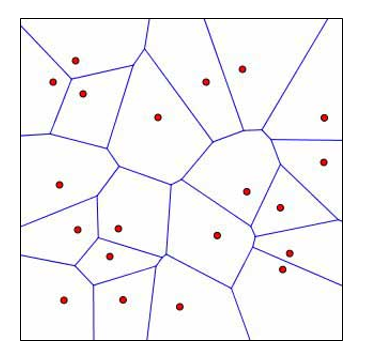
\includegraphics[scale=0.5]{voronoiExample.PNG}
                    \caption{Voronoi diagram example}
                \end{center}
            \end{figure}

            The complexity of k-NN algorithm is same to Voronoi Diagram for $k$ dimensions.

            In 2 dimension, the case of Voronoi Diagram, using efficient data structures such as a binary search tree to find the nearest neighbors, it can be shown that the computational efforts involved are proportional to depth of the tree which is \(\approx \log(N)\) where $N$ is the number of data points or nodes stored in the tree. 

            Extending this concept to multiple dimensions, one can use k-d tree. Given a balanced binary tree (starting from the median for example), it can be shown that the computational complexity is of the order $kp\log(N)$ where, $k$ is the number of classes, $p$ is the number of features and $N$ is the number of data points. 

            With this analysis, one can comment on the limitations and applicability of k-NN. The method is clearly effective if $k$ and $p$ is small compared to number of data points $N$. This makes it extremely effective for on-line learning. Additionally, it is clear that k-NN is not effective if number of features is large. 
        }

        \paragraph{High dimension distance}{
            Considering a one dimensional problem and the space is bound between 0 and 1. Let us generously assume that even 0.99 is \textit{near} to 0. In other words, 99\% of the space is close to 0. 

            If we scale it up to 2 dimensions, this '\textit{near}' region becomes \(\mathrm{0.99^2} \approx \mathrm{0.98}\). 

            Extending it to just 1000 dimensions, this region becomes \(\mathrm{4.3 x 10^{-5}}\). Which means in 1000 dimension one needs approximately 23000 points to get same 'density' of points as one would get with just 1 point in 1 dimension. So hard to find near points.

            Generally, we keep the rule that: \(N\gg 2^p\), \(N \rightarrow \) Numbers of points, \(P \rightarrow features\)
        }
    }
    \subsection{Standardization}{
        \paragraph{e.g. Scale dependence}{
            Given 3 data points, which describe the age and salary, as follows:

            $a$ = (45, \$76000), $b$ = (25, \$75000), $c$ = (42, \$78000). 

            If we choose Eucliden distance as the measure, \(\mathrm{d}(a, b) = \|a - b\| = \sqrt{\mathrm{20^2} + \mathrm{1000^2}} \approx 1000\). Similarly, $\mathrm{d}(b,c) \approx$ 3000 and $\mathrm{d}(a,c) \approx$ 2000.

            Changing the scale of salary by a factor of 1000, then the distance can be written in $\mathrm{d}(a, b) = \|a - b\| = \sqrt{\mathrm{20}^2 + \mathrm{1}^2} \approx$ 20. Similarly, $\mathrm{d}(b,c) \approx$ 17 and $\mathrm{d}(a, c) \approx$ 3.6.

            Thus, scale in which data is reported can affect selection of nearest points and this makes outcome of k-NN scale dependent. 
        }
        Assuming that the data roughly follows a normal distribution, 

        \[\utilde{x} \rightarrow x_1, x_2,\cdots,x_n\] 

        Standardize: \(x_k = \frac{x_k - \bar{X}}{s}\) 

        where \(\bar{X} =\frac{\sum_{i=1}^{n}x_i}{n}\) is the mean, and \(s = \frac{\sqrt{\sum_{i=1}^{n}(x_i - \bar{X})^2}}{n-1}\) is the standard deviation.

        One point notice in case of this standardization is that this approach is effective only when features are completely independent of each other. If the features are correlated, one might end up overemphasizing some of the features and under-emphasizing some. 

        To avoid this, use of a covariance matrix is suggested. Covariance matrix $\mathbb{S}$ is defined as \[\mathbb{S}_{ij} = \sum_l(x_{il} - \bar{x_i})(x_{jl} - \bar{x_j})\]
        \[x_i \rightarrow (x_i - \bar{X}\cdot \utilde{i})^T\mathbb{S}^{-1} (x_i - \bar{X}\cdot \utilde{i})\]. 

        In which use \(\bar{X}\cdot \utilde{i}\) to vectorize the \(\bar{X}\).

        Therefore, \(d(a, b) = \sqrt{(a - b)^T \mathbb{S}^{-1}(a - b)}\). 

        If the correlation is large intuitively, \(\mathbb{S}^{-1}\) becomes small and it weighs down the distance. As a result of these computations, evaluating \(\hat{f}\) at a new point is expensive.
    }
}

\end{document}
